\documentclass{subfiles}
\begin{document}
\section{Implementation summary and workflow}\label{sec:summary_workflow}
Having now introduced the theoretical background and numerical strategies used to solve the time-dependent Schrödinger equation (TDSE) for our Morse double well quantum dot system, we conclude this chapter with a brief summary of how the various numerical components fit together in practice. This overview outlines the structure of our simulation codebase and the logic behind the implementation. The goal is to clarify how the different parts interact to evolve the quantum state over time and realise the quantum time evolution. 
\subsection*{Structure of the simulation framework}

The simulation pipeline in this thesis follows a logical sequence, designed around the Morse double-well potential system for two interacting particles. The key stages of the implementation are as follows:
\begin{enumerate}
    \item \textbf{Construct the Morse double-well potential} \\
    The first step is to implement a flexible and numerically stable representation of the Morse potential \eqref with a double-well structure. This involves defining the functional form of the potential, setting physical parameters (well separation, depth, width), and discretizing the spatial domain to represent the wavefunctions and operators. 

    \item \textbf{Setup of the Hamiltonian matrix} \\
    In our Sinc-DVR basis, we compute all one-body (kinetic + potential) and two-body (Coulomb) integrals to set up our full two-particle Hamiltonian matrix (Section \ref{sec:sinc_dvr_validation}). We then construct the Hartree matrices for the two subsystems, which are used to diagonalize the system and project the full Hamiltonian onto a smaller subspace that accurately captures the essential dynamics of our system.

    \item \textbf{System preparation} \\
    A separate optimization routine searches for two target configurations - $C_I$, in which the wells have well-separated, non-degenerate transition energies, and $C_{II}$, where the first excited states of the two subsystems are nearly degenerate. Once the optimal parameters are found, we rebuild the Hartree basis at $C_I$ and use this basis throughout the evolution for consistent overlap calculations.

    \item \textbf{Time discretization and ramp protocol} \\
    We lay down a uniform time grid with step size $\Delta t$ over a total time $T$. On that grid we specify a ramping protocol that linearly interpolates the potential parameters from $C_I$ to $C_{II}$ and back at a chosen speed, staying entirely within the initial Hartree basis. 

    \item \textbf{Time-propagation} \\
    We then evolve the quantum state using one of two interchangable propagators - either direct matrix exponentition of the Hamiltonian, or the implicit Crank-Nicolson time integrator. Choice of method depends on the specific requirements of the simulation.

    \item \textbf{Post-processing and analysis} \\
    After time evolution, we overlaps and state populations, von Neumann entropies, and other physical observables of interest. We also compute the unitary matrix $U$ that represents the time-evolved gate operation, and apply phase correction single-qubit rotations before computing gate fidelity measures to assess the performance of our quantum gate. 
\end{enumerate}
\subsection*{Summary}

The overall workflow — from system definition to result analysis — closely mirrors the physical logic of quantum simulation:
\begin{enumerate}
    \item Build the system (basis + Hamiltonian),
    \item Prepare the system (potential parameters),
    \item Define the time domain and control fields,
    \item Evolve the state using a suitable propagator,
    \item Correct for any phase misalignments,
    \item Extract and analyze physical quantities of interest.
\end{enumerate}

This structure provides a coherent and extensible framework for studying both fundamental quantum dynamics and more complex qubit-like behavior in the coupled double-well Morse potential system.

\begin{figure}[h!]
    \centering
    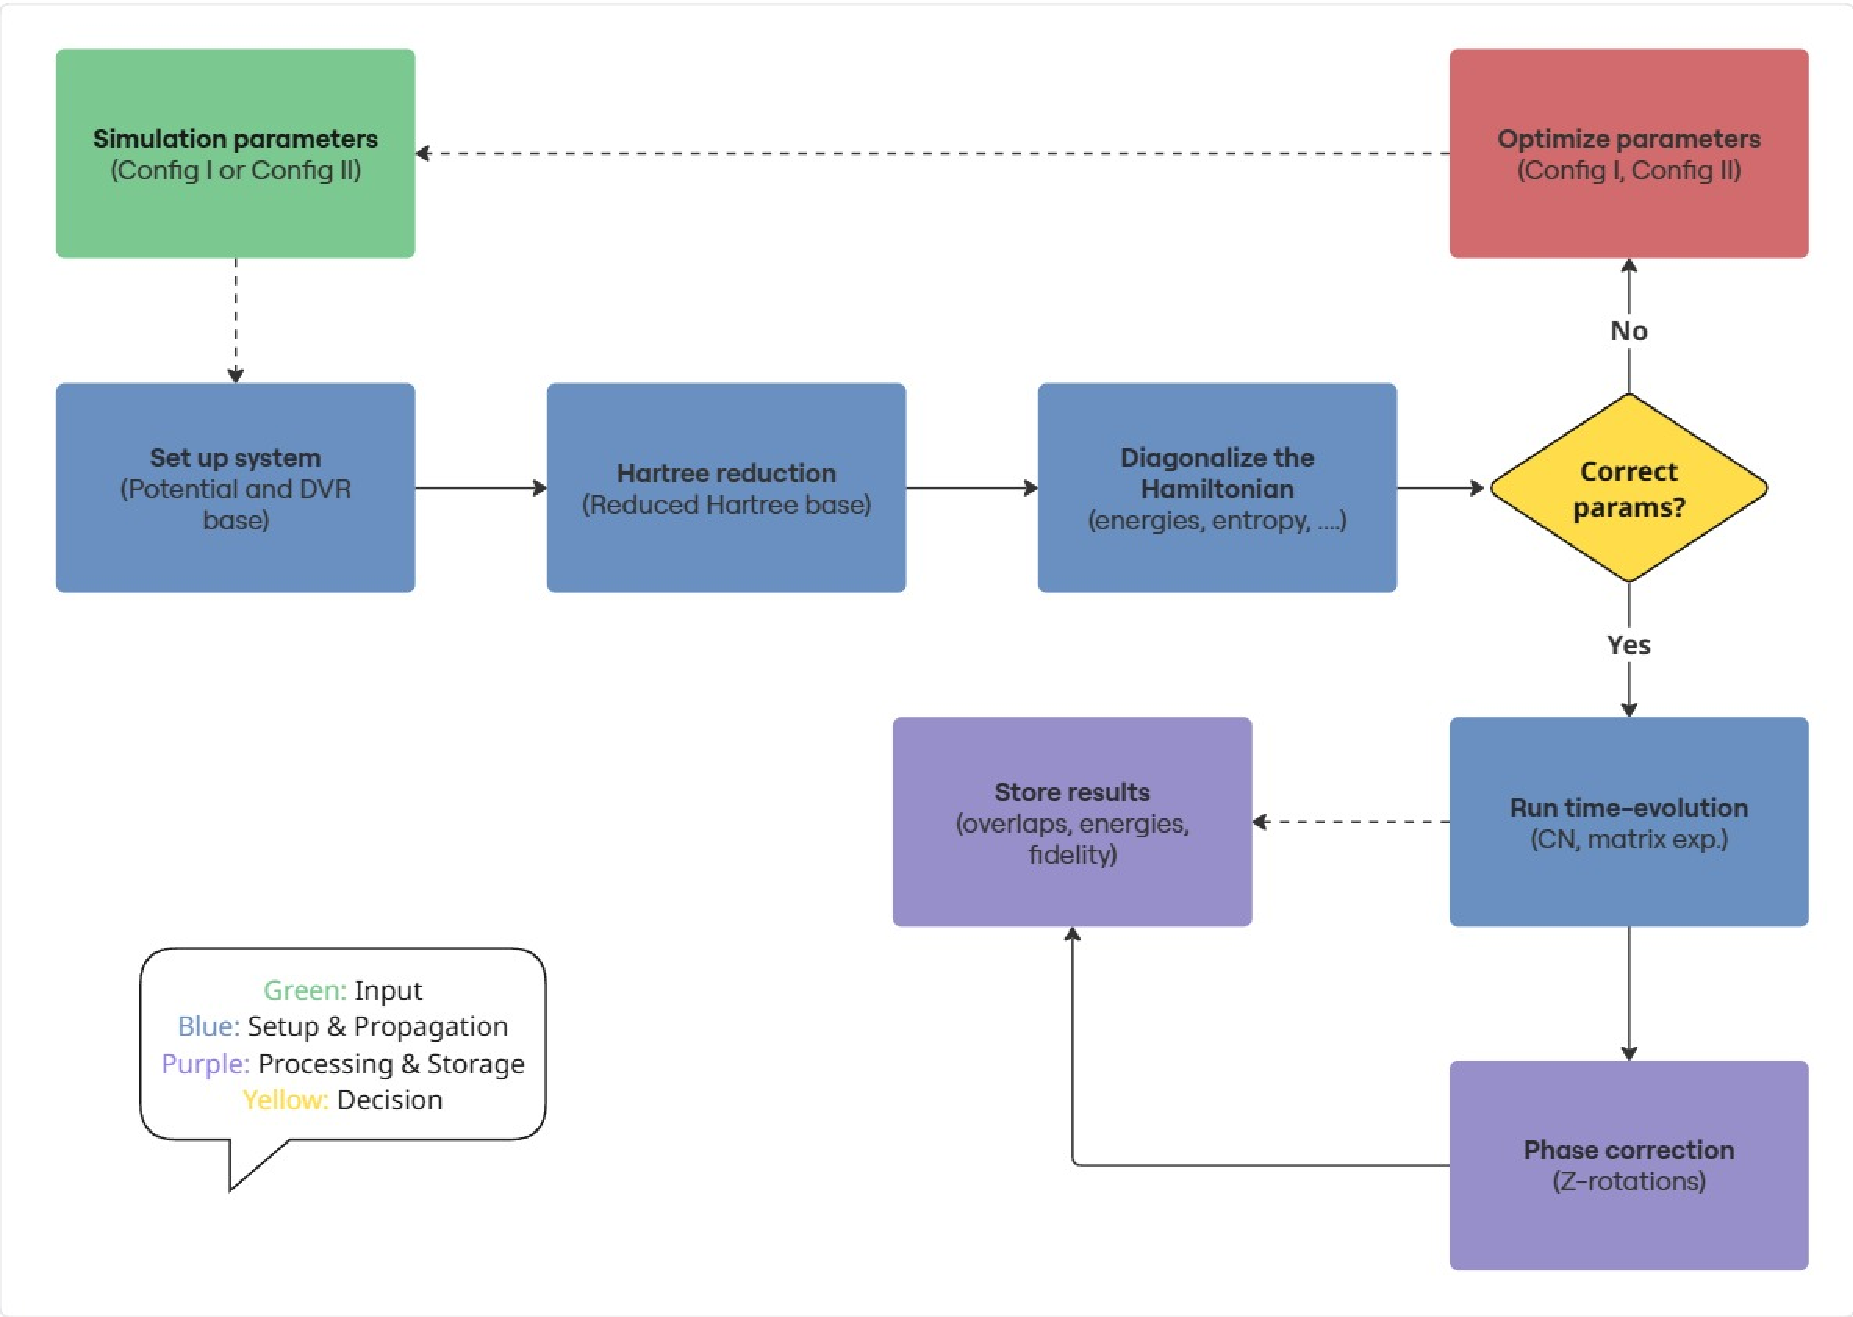
\includegraphics[width=1.0\textwidth]{figs/Flowchart.pdf}
    \caption{Graphical overview of the numerical workflow for simulating the two-particle Morse double-well potential system. The flowchart illustrates the main components of the simulation, from system setup and optimization, through time evolution and post-processing and gate fidelity calculations. }
\end{figure}

\end{document}